\documentclass{article}

\usepackage{aaai/aaai}
\usepackage{algorithm}
\usepackage{algorithmic}
\usepackage{amssymb}
\usepackage{enumerate}
\usepackage{fullpage}
\usepackage{graphicx}
\usepackage{psfrag}
\usepackage{tikz}
\usepackage{times}

\usetikzlibrary{intersections}

\newtheorem{theorem}{Theorem}
\newtheorem{lemm}{Lemma}
\newtheorem{defi}{Definition}
\newenvironment{proof}{\noindent{\bf Proof:}}{\hspace{\stretch{1}}$\Box$\vspace{0.5em}\newline}

\newcommand{\intersection}[2]{\langle #1, #2\rangle}
\newcommand{\anya}[0]{{\bf anya}}

\newcommand{\creategrid}[2]{%
  \draw[step=1] (0,0) grid (#1,#2);%
%
  \foreach \x in {1,...,#1}%
    \draw (\x - 0.5, -0.5) node {\x};%
%
  \foreach \y in {1,...,#2}%
    \draw (-0.5, \y - 0.5) node {\y};%
}%
\newcommand{\drawobstacle}[2]{%
\draw[fill=black] (#1,#2) rectangle +(-1,-1);
}%


\begin{document}

\title{An Optimal Any-Angle Pathfinding Algorithm}
\author{Paper Id: 14}

\maketitle

\chapter{Introduction}
\label{cha::intro}

Pathfinding is the name given to a broad class of related problems
often appearing in Computer Science. In the canonical case the
pathfinding problem asks that we navigate between an arbitrary pair of 
start and target locations drawn from a map. Such problems
appear in a myriad of important and real-life contexts. For example:
\begin{itemize}
\item Pathfinding is at the heart of all personal GPS navigation devices.
\item Pathfinding is used by transportation and logistics companies to 
improve performance and reduce operating costs.
\item Pathfinding is central to the correct operation of personal and industrial robots.
\item Pathfinding powers the AI systems of many modern computer games.
\end{itemize}

\noindent Just as there are many possible application areas for pathfinding there are
equally many variations of the problem as well. Frequently we are
asked to find a path which is optimal with regard to distance. In other cases
a more desirable path can be one that minimises travel time or even travel
cost.  Sometimes it may not necessary -- or even possible -- to compute an
optimal path: low-power or real-time computing devices place
strict limits on the amount of resources (CPU, memory) that are available for
navigation.  In these cases near-optimal, bounded sub-optimal or indeed any
path at all will often suffice. Other types of pathfinding problems include
(but are not limited to) finding a path in a dynamic environment, finding a path 
in three or more dimensions, navigating in the presence of other moving entities and
even chasing a moving target. All these topics have received 
extensive attention from both researchers and industrial practitioners.

In this thesis we will aim to compute distance-optimal paths in a discrete
and static two-dimensional environment. Our target applications are robotics and computer games.
We will study a range of different approaches but in each case our objective will
be (i) to find the shortest path, (ii) as quickly as possible and (iii) as economically
as possible with respect to available resources such as memory and pre-computation time. 


\section{Introduction}
Any-angle pathfinding is a navigation problem which appears in robotics
and computer video games. It involves finding a shortest path between an 
arbitrary pair of points on a two-dimensional grid map but asks that 
movement along the path is not artificially constrained to the points of 
the grid.  Within the game development community a simple and popular 
solution exists known as \emph{string pulling}~\cite{pinter01,botea04}.
The idea is to compute a grid-optimal path in the first
instance and smooth the result as part of a post-processing step that improves
both its length and aesthetic appeal. String pulling has two disadvantages: 
(i) it requires more computation than just finding a path (ii)
it only yields approximately shortest paths.

A number of algorithms improve on string-pulling by integrating post-processing
into node-expansion during search. Field D*~\cite{ferguson05} uses linear 
interpolation to smooth paths one grid cell at a time. 
Theta*~\cite{nash07} 
%and its variants %\cite{%nash09, nash10,munoz12}
introduces a shortcut each time a successful line-of-sight check
is made from the parent of the current node to any of its successors.
Meanwhile, Block A*~\cite{yap11} employs during search a pre-computed database
of optimal Euclidean distances between pairs of points in a localised area.
Each of these approaches improves on string pulling in terms of solution 
quality and, in many cases, running time. Unfortunately none are optimal.
Accelerated A*~\cite{sislak09b} is an any-angle algorithm that is conjectured 
to be optimal but for which no strong theoretical argument is made. Similar to Theta*, 
it differs primarily in that line-of-sight checks are performed from a set
of expanded nodes rather than a single ancestor. The size of the set is only
loosely bounded and, for challenging problems, can include a large proportion
of nodes on the Closed List.

%
% Its main disadvantage is that,
%for challenging problems, it can perform line-of-sight checks against a large 
%proportion of nodes on the Closed List.
%
%Theta*~\cite{nash07} and its variant~\cite{%nash09,
%nash10} improve things 
%by integrating post-processing into node expansion during search. Their 
%idea involves updating a node's parent label following a successful line-of-sight
%check to a previously expanded ancestor node.
%Another approach, Block A*~\cite{yap11}, avoids line-of-sight checks entirely 
%by precomputing a database of exact costs between pairs of points in a localised area.
%Both Theta* and Block A* improve on the running time and 
%solution quality of string pulling but neither guarantees optimality.
%Despite this, a number of exact solutions for the problem do exist.
%\\
%In computational geometry a problem similar to any-angle pathfinding exists 
%which has been very well studied: finding Euclidean shortest paths among 
%polygonal obstacles in the plane.
Tangent Graphs~\cite{liu92} and Visibility Graphs~\cite{lozanoperez79} are 
optimal techniques that can solve a generalised form of the any-angle pathfinding 
problem. Their primary disadvantage is that each such graph requires quadratic 
space in the worst case and must be computed offline.
Other exact approaches are based on the 
Continuous Dijkstra~\cite{mitchell87} paradigm.
The most efficient of these algorithms~\cite{hershberger99} pre-computes a 
planar subdivision of the map that can be used to extract a path in just
logarithmic time. Unfortunately the precomputation assumes the starting location
does not change.

In this work we introduce a new approach to any-angle pathfinding 
which addresses many of the shortcomings associated with existing research.
Our method, Anya, bears some similarity with Continuous Dijkstra: 
instead of searching over the individual nodes of the grid we 
search over contiguous sets of states that form intervals.
Each interval has a representative point used to derive an $f$-value
and each is projected from one row of the grid onto another until the 
goal is reached.
%instead of searching over individual states from the grid we consider
%contiguous sets of states together as an interval. From each interval we select a 
%representative point that is used to derive an $f$-value for the set.
%Intervals are associated with corner points and projected from one 
%row of the grid onto another until the goal is reached.
Anya does not rely on any precomputation, does not introduce any
memory overheads (beyond what is required by e.g. A*) and always finds 
an optimal any-angle path.
%compares favourably with existing research: (i)
%it always finds an optimal any-angle path (ii) 
%it does not rely on any precomputation (iii) 
%it does not introduce any memory overheads 
%beyond those required by a pathfinding algorithm such as A*.

%http://www.valvesoftware.com/publications/2009/ai_systems_of_l4d_mike_booth.pdf
%http://digestingduck.blogspot.com.au/2010/03/simple-stupid-funnel-algorithm.html

\begin{itemize}
\item 
  Grid.  
\item 
  Corner (of an obstacle).  
\item 
  Grid point.  
  $\intersection{x}{y}$.  
\item 
  Visibility of point from a point.  
\item 
  Any-angle path and turning point.  
\item 
  Interval $[p,p']$.  
\end{itemize}

\begin{lemm}
  In an optimal any-angle path, 
  a turning point is a corner.  
\end{lemm}

% EOF

\section{Principle Of Anya}
Consider as a motivating example the problem depicted in Figure~\ref{fig::ex1}.
We are tasked with finding an any-angle path between node $n_1 = (2, 0)$ and
node $n_2 = (3, 4)$.  The best online algorithm for solving this problem, to
date, is Theta*~\cite{nash07}. It operates by looking for a solution among the
set of discrete points that comprise the locations of the grid; i.e.,
it successively expands nodes $(2,1)$ to $(2,4)$ and $(3,0)$ to $(3,3)$ until
eventually $n_2$ is reached.  Notice however that the actual shortest path
between $n_1$ and $n_2$ may not pass through any of these discrete points.  To
account for this fact Theta* ``pulls the string'' each time a new
point is reached.  Thus when node $n_2$ is generated its $g$-value is not
computed as the length of the grid-constrained path used to reach it but rather
using the direct path $\langle n_1, n_2 \rangle$.

%\begin{figure}[tb]
% \begin{minipage}[b]{\0.45\linewidth}
%  \begin{center}
%    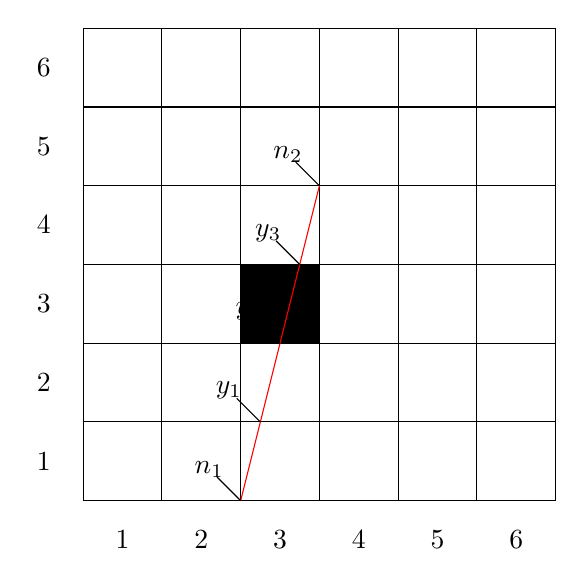
\begin{tikzpicture}

\creategrid{6}{6}

\drawobstacle{3}{3}

\coordinate (n1) at (2,0);
\coordinate (n2) at (3,4);

\path[name path=direct] (n1) -- (n2);
\path[name path=row 1] (0,1) -- (6,1);
\path[name path=row 2] (0,2) -- (6,2);
\path[name path=row 3] (0,3) -- (6,3);
\draw[name intersections={of=direct and row 1,by=y1}];
\draw[name intersections={of=direct and row 2,by=y2}];
\draw[name intersections={of=direct and row 3,by=y3}];

\draw[red] (n1) -- (n2);

\draw (n1) ++(-0.4,0.4) node {$n_1$} + (0.1,-0.1) -- (n1);
\draw (n2) ++(-0.4,0.4) node {$n_2$} + (0.1,-0.1) -- (n2);
\draw (y1) ++(-0.4,0.4) node {$y_1$} + (0.1,-0.1) -- (y1);
\draw (y2) ++(-0.4,0.4) node {$y_2$} + (0.1,-0.1) -- (y2);
\draw (y3) ++(-0.4,0.4) node {$y_3$} + (0.1,-0.1) -- (y3);

\end{tikzpicture}

%  \end{center}
%  \caption{Example of an any-angle path}
%  \label{fig::ex1}
%  \end{minipage}
%\end{figure}

The problem with this approach is that the solution-cost estimate
(or $f$-value), from a parent node to each of its successors, may 
not be monotonically increasing.  The monotone condition is
necessary to guarantee that an optimal solution, if one exists, is always found.
For instance: Theta* can generate $n_2$ from the intermediate point $p = (3,3)$.
When $p$ is expanded we have $f(p) = d(n_1, p) + h(p, n_2) = 4.16$. 
To satisfy the monotone condition we require that $f(n_2) \geq 4.16$. However 
Theta* computes $f(n_2) = d(n_1, n_2) + h(n_2, n_2) = 4.12$.
Clearly $p$ should be expanded after $n_2$ but in this case the opposite occurs.  
In order to avoid this mistake we would need to consider, in addition to the
set of discrete points from the grid, all the points $y_i$ shown in Figure~\ref{fig::ex1}.
The problem is that the number of such points can be very large:
each edge of the grid, together with its discrete endpoints, 
forms a $[0, 1]$ interval that can be intersected by the optimal
path at any point $0 \leq \frac{w}{h} \leq 1$; here $w$ (resp. $h$) is an integer in
$\{0,\dots,W\}$ (resp.  $\{0,\dots,H\}$).
This is a set whose members are reducible to a Farey Sequence.
For any given $n$ (in our case $n = \max(W, H)$) the cardinality of the corresponding 
set of elements is known to be quadratic in $n$~\cite{concrete89}.
We are therefore motivated to consider an alternative approach: instead
of evaluating each $y_i$ node individually we will evaluate together
all the nodes from the corresponding interval in which each $y_i$ appears.



\section{Algorithm}
%The best online approaches for any-angle pathfinding consider 
%only the set of discrete points that define the grid.
%Since this strategy is insufficient to guarantee optimality 
%we will consider sets of discrete and intermediate points
%by taking them together as an interval.

\begin{defi}
\label{defi::interval}
A \emph{grid interval} $I$ is a set of contiguous pairwise
visible points found along any row of the grid. 
Each interval can be described in terms of its endpoints $a$
and $b$.
\end{defi}
We will say that an interval $I = (a, b)$ is open (resp. $I = (a, b]$ is half-open) if both 
of its endpoints (resp. $a$) is the start or target location or 
a discrete corner point. 
$I = [a, b]$ can also be closed in which case $a = b$ is
a single discrete location: the start point, the target point
or a discrete corner point. 
We do not allow an open (resp. half-open) interval to contain a 
sub-interval which is closed.
\begin{defi}
A \emph{search node} $n = (I, r)$ is a tuple where $I$ is an interval and $r$
is a \emph{root} point chosen such that each $p \in I$  is visible from $r$. 
The identity of the root node is either the start location or the most
recent corner point on the path used to reach $I$.
\end{defi}
We will look for optimal any-angle paths in the search space formed by
intervals appearing along the rows of the grid.
To evaluate a search node $n = (I, r$) we will use a single representative 
point $p \in I$ which has a minimum $f$-value with respect to a target point
$t$:
\begin{equation}
f(n) = \arg\min \lbrace f(p) = g(r) + d(r, p) + h(p, t) \rbrace 
\end{equation}
Although each interval can contain a large number of points it is easy
to identify the one having a minimum $f$-value: 
we simply project a straight line $r \rightarrow t$ from the root point $r$ to the 
target $t$ and choose the point $p \in I$ which is intersected by the line.
In the case that $r \rightarrow t$ does not intersect any point in $I$ we simply
choose the endpoint of $I$ closest to $t$. 
In the following we give a formal argument that this strategy always identifies
$p \in I$ having a minimum $f$-value.

\begin{lemm}
A true statement will go here.
\end{lemm}
\begin{proof}
A very clever and convincing proof will go here.
\end{proof}
%
%Our search nodes will comprise of tuples of the form $(I, r)$ where
%$I$ is an interval and $r$ is a \emph{root} point which can be
%either the start location or the most recent corner point on the path used
%to reach to $I$.
%Given any such tuple we require that each $p \in I$ is visible from $r$.
%\\
During search we will project intervals from one row of the grid to another.
In particular we will say that the successors of an interval $I$
are just those intervals $I'$ which are immediately adjacent
to $I$.
\begin{defi}
\label{defi::intadj}
A grid interval $I$ is \emph{adjacent} to $I'$ iff for every pair 
of points $p \in I$ and $p' \in I'$ there exists a straight line
path that does not pass through any interval 
$J \not \in \lbrace I, I' \rbrace$
\end{defi}
Definition~\ref{defi::intadj} bounds the branching factor of each 
search node to $O(W)$ and unlike other exact algortihms (e.g. visibility graphs)
allows us to defer the generation of any neighbours that are not 
immediately promising.
\\

\section{Stuff that is not finished}

Essentially, the reason why the existing algorithms are not optimal
is that the search is based on the grid intersections.  
However, because the final any-angle path 
may never cross these intersections, 
the $A^*$ $f$ value associated with the intersections
is not relevant.  
In this article, we propose to run the search not on the grid 
but instead on the edges of the graph.  

bla bla

From $n_1$, all the nodes that can be reached with a one step North 
(and potentially any fraction of West/East steps) will be considered.  
We call ``interval'' this set of nodes that are considered together.  

How should we then compute the successors of an interval?  
Look at Figure~\ref{fig::succ1} (left) 
where a North step is taken from the interval $[(1,3)-(4,3)]$
reached from node $(1,1)$.  
The (single) successor of the interval 
is simply computed by projecting the visibility cone 
(represented with dashed lines)
from $(1,1)$ to the next row.  
This leads to the interval $[(1,4)-(5+\frac{1}{2},4)]$.  
Obverse that, as a consequence, the parent of the interval 
(here $(1,1)$) must be kept together with the interval.  

\begin{figure}[ht]
  \begin{minipage}{0.5\linewidth}
  \begin{center}
    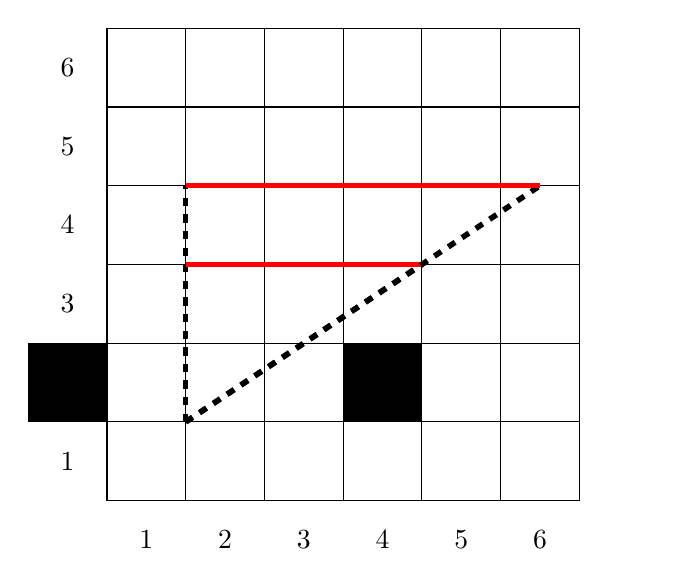
\begin{tikzpicture}

\creategrid{6}{6}
\drawobstacle{0}{2}
\drawobstacle{4}{2}

\draw[dashed, line width=2] (1,1) -- (1,4);
\path[name path=p1] (1,1) -- +(6,4);
\path[name path=p2] (0,4) -- (6,4);
\path[name path=p3] (0,3) -- (6,3);

\draw[name intersections={of=p1 and p3,by=x2}];
\draw[dashed, line width=2] (1,1) -- (x2);
\draw[red,line width=2] (1,3) -- (x2);

\draw[name intersections={of=p1 and p2,by=x1}];
\draw[dashed, line width=2] (1,1) -- (x1);
\draw[red,line width=2] (1,4) -- (x1);

\end{tikzpicture}

  \end{center}
  \end{minipage}
  \begin{minipage}{0.5\linewidth}
  \begin{center}
    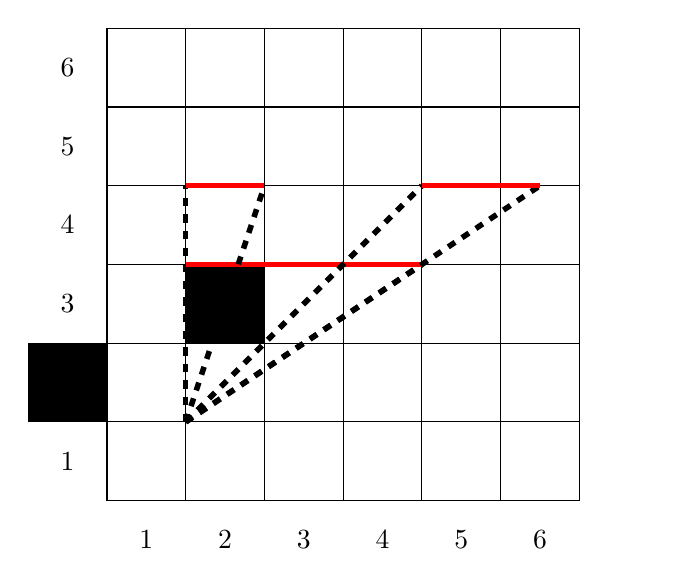
\begin{tikzpicture}

\creategrid{6}{6}
\drawobstacle{0}{2}
\drawobstacle{2}{3}

\draw[dashed, line width=2] (1,1) -- (1,4);
\path[name path=p1] (1,1) -- +(6,4);
\path[name path=p2] (0,4) -- (6,4);
\path[name path=p3] (0,3) -- (6,3);
\path[name path=p4] (1,1) -- +(4,4);

\draw[name intersections={of=p1 and p3,by=x2}];
\draw[dashed, line width=2] (1,1) -- (x2);
\draw[red,line width=2] (1,3) -- (x2);

\draw[name intersections={of=p1 and p2,by=x1}];
\draw[dashed, line width=2] (1,1) -- (x1);
\draw[red,line width=2] (1,4) -- (2,4);
\draw[dashed, line width=2] (1,1) -- (2,4);
\draw[name intersections={of=p4 and p2,by=x3}];
\draw[dashed, line width=2] (1,1) -- (x3);
\draw[red,line width=2] (x3) -- (x1);

\end{tikzpicture}

  \end{center}
  \end{minipage}
  \caption{Computing the successors of an interval}
  \label{fig::succ1}
\end{figure}

There are more complicated situations, 
as presented in Figure~\ref{fig::succ1} (right).  
Here, we can see that an obstacle splits the interval 
in two separate intervals.  
We could define disjunct intervals, 
but it seems more natural to consider them independently.  

Furthermore, the path might turn at node $(3,3)$
(e.g., to reach node $(3,4)$
which is not directly accessible from $(1,1)$).  
The corner $(3,3)$ is therefore a successor of node $(1,1)$ 
and intervals should be built from this node.  

%Let us present more precisely how the successors are splitted.  
%From the interval $I = [(1,3)-(4,3)]$, 
%we assume that an epsilon step 
%(i.e., an infinitely small step North) is taken.  
%This step reveals how the interval will be splitted.  
%Therefore, we generate interval 
%$[(1,3+\varepsilon)-(4+\frac{3}{2}\varepsilon,3+\varepsilon)]$; 
%we then remove the parts that belong to the obstacle, 
%which produces the two intervals 
%$[(1,3+\varepsilon)-(2,3+\varepsilon)]$ 
%$[(3,3+\varepsilon)-(4+\frac{3}{2}\varepsilon,3+\varepsilon)]$; 
%finally, we split the part that is not visible from $(1,1)$, 
%which leads to three intervals: 
%$[(1,3+\varepsilon)-(2,3+\varepsilon)]$, 
%$[(3,3+\varepsilon)-(3+\varepsilon,3+\varepsilon)]$, 
%and
%$](3+\varepsilon,3+\varepsilon)-
%(4+\frac{3}{2}\varepsilon,3+\varepsilon)]$. 
%If we project back on row 3, 
%we obtain three intervals: 
%$[(1,3)-(2,3)]$, 
%$[(3,3)-(3,3)]$, 
%and
%$](3,3)-(4,3)]$. 
%We say that these intervals are ``consistent''%
%\footnote{We need a better word here.} 
%with the obstacles.  
%The first and last intervals can be delt with similarly 
%to the example in Figure~\ref{fig::succ1} (left).  
%The second interval, being a single point, 
%requires to generate new intervals.  

The remaining question is what $f$ value 
should be associated with these intervals.  
For $A^*$ to return the optimal solution, 
we need $f$ to be an underestimate of the actual value 
(except for the final node).  
The interval has the following semantics: 
the path that is currently being constructed 
should start from $s$, cross the parent $P$, 
then cross the interval, and finally reached the goal.  
The shortest path that belongs to this set 
has length $g^*(P) + min_{x \in I}(d(P,x) + h^*(x))$.  
The value $g^*(P)$ should be known at this stage 
(this is one advantage of $A^*$).  
However, the minimum factor is unknown, 
but it can be lower-bounded by $min_{x \in I}(d(P,x) + h(x))$.  
This formula is actually pretty simple to solve, as we now demonstrate.  

Let $z_1$ and $z_2$ be the two extreme points of the interval.  
Draw a direct line between the goal and the parent $P$ of the interval, 
as shown in Figure~\ref{fig::fvalue}.  
If the line crosses the interval in \textit{\u z}, then the value is h(P).  If the line passes on the left, 
then the value is $d(P,z_1)+h(z_1)$; 
otherwise, it is $d(P,z_2)+h(z_2)$.  
If the goal is between the parent and the interval, 
as is the case with $g_4$, 
then one needs to consider the mirrored version of $g_4$ 
(here $g'_4$).  

\begin{figure}[ht]
  \begin{center}
%    \includegraphics[scale=0.3]{images/fvalue}
    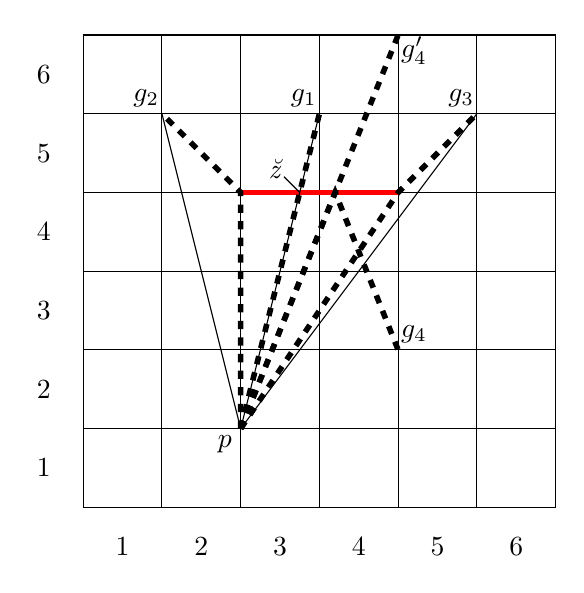
\begin{tikzpicture}

\creategrid{6}{6}
%\drawobstacle{2}{3}

\draw[red,line width=2] (2,4) -- (4,4);

\coordinate (root) at (2,1);
\coordinate (g1)   at (3,5);
\coordinate (g2)   at (1,5);
\coordinate (g3)   at (5,5);

\foreach \g in {g1, g2, g3}
  \draw (root) -- (\g);

\path[name path=direct] (root) -- (g1);
\path[name path=interval] (2,4) -- (4,4);
\draw[name intersections={of=direct and interval,by=zsmile}];
\draw (zsmile) -- ++ (-0.2,0.2) + (-0.1,0.1) node {\textit{\u z}};

\draw[dashed,line width=2pt] (root) -- (g1);
\draw[dashed,line width=2pt] (root) -- (2,4) -- (g2);
\draw[dashed,line width=2pt] (root) -- (4,4) -- (g3);

\draw (g1)   + (-0.2,0.2) node {$g_1$};
\draw (g2)   + (-0.2,0.2) node {$g_2$};
\draw (g3)   + (-0.2,0.2) node {$g_3$};
\draw (root) + (-0.2,-0.2) node {$p$};

\coordinate (g4)   at (4,2);
\draw (g4)   + (+0.2,0.2) node {$g_4$};
\coordinate (g4mirror) at (4,6);
\draw (g4mirror) + (+0.2,-0.2) node {$g'_4$};
\path[name path=directtwo] (root) -- (g4mirror);
\draw[name intersections={of=directtwo and interval,by=zsmiletwo}];
\draw[dashed,line width=2pt] (root) -- (zsmiletwo) -- (g4);
\draw[dashed,line width=2pt] (root) -- (g4mirror);

\end{tikzpicture}

  \end{center}
  \caption{Computing the minimum distance 
    to go from $p$ through the interval to the goal; 
    if the goal is $g_1$, the direct distance between $p$ and $g_1$; 
    if the goal is $g_2$ or $g_3$, 
    the shortest distance is the distance represented by the dashed lines.}
  \label{fig::fvalue}
\end{figure}

% EOF
This section now presents our search algorithm, dubbed \anya, short for
any-angle pathfinding.  \anya{} is a variant of A* that does not search on the
space of intervals of the grid, but instead on the space of intervals and
corners.

\begin{algorithm}[ht!]
  \begin{algorithmic}
\STATE {\bf input}: Graph $G$, source $s$, target $t$
\STATE $open := \{s\}$
\LOOP
  \STATE $i := pop(open)$
  \IF{$i = t$}
    \STATE {\bf return} $i$
  \ENDIF
  \IF{$i$ is a node}
    \FORALL{$i' \in$ successors\_of\_corner($i$)}
      \STATE add\_edge($i$,$i'$)
    \ENDFOR
  \ELSE %\COMMENT{$i$ is an interval}
    \STATE {\bf let} $i = \langle [x_{\min},x_{\max}],y,p\rangle$.
    \STATE $i_1 :=$ move($i$)
    \STATE $cs :=$ corners\_of($i_1$)
    \COMMENT{Including target.}
    \STATE $is :=$ split($i_1,cs$)
    \FORALL{$c' \in cs$}
      \IF{$c'$ is visible from $p$}
        \STATE add\_edge($i$,$c'$)
      \ENDIF
    \ENDFOR
    \FORALL{$i' \in is$}
      \STATE {\bf let} $i' = \langle [x'_{\min},x'_{\max}],y',p\rangle$.
      \IF{$\langle \frac{x'_{\min}+x'_{\max}}{2},y'\rangle$ is visible from $p$}
        \STATE add\_edge($i$,$i'$)
      \ENDIF
    \ENDFOR
  \ENDIF
\ENDLOOP
\end{algorithmic}


  \caption{Procedure \anya, an any-angle pathfinding algorithm}
  \label{algo::anya}
\end{algorithm}

The general layout of \anya{} is given in Algorithm~\ref{algo::anya}.  
Like A*, \anya{} keeps a priority queue called $open$ 
and based on the $f$ value.  
The algorithm stops when the target is poped from the queue.  
Now, whether the current node is a corner or an interval 
is dealt with differently by \anya: 
\begin{itemize}
\item 
  For a corner, the successors of the corner are computed 
  (method successors\_of\_corner presented later) 
  and are added to the priority queue --- 
  the method add\_edge deals with computing the $f$ value 
  (presented later), updating if necessary the parent of a node, 
  and sorting the priority queue.  
\item 
  If the node is an interval, \anya{} moves it 
  and computes the corners of the new interval 
  (for this purpose, the target is seen as a corner).  
  Then, the interval is split according to the corners, 
  i.e., producing all the intervals between two consecutive corners.  
  All these corners and intervals 
  are potential successors of the current interval; 
  however, we need to check that they are visible from parent $p$.  
  To check whether an interval is visible, 
  we check whether its middle point is.  
\end{itemize}

We illustrate the computation of the successors 
of interval $i = \langle [1,2],3,p\langle$ 
where $p = \langle1,1\rangle$ 
(cf. Figure~\ref{fig::succ1}, right).  
The move of $i$ produces 
the interval $i' = \langle [1,2.5],4,p\rangle$.  
The set of corners of $i'$ is $\{\langle 2,4\rangle\}$.  
The split of $i'$ hence produces two intervals: 
$is = \{
\langle [1,2],4,p\rangle,  
\langle [2,2.5],4,p\rangle
\}$.  
The single corner is visible from $p$.  
The point $c' = \langle 1.5,4\rangle$ is also visible from $p$, 
which means that the first interval is visible from $p$.  
On the other hand, the point $\langle 2.25,4\rangle$ 
is not visible from $p$, 
which means that the second interval is not visible from $p$.  
The successors of $i$ are therefore $c'$ 
and $\langle [1,2],4,p\rangle$.  

\paragraph*{}

A corner $\langle x,y\rangle$ has potentially four successors.  
The first two obvious successors 
are the intervals at rows $y-1$ and $y+1$.  
However, the optimal path may follow a horizontal section, 
and the corner could have a successor on the left or on the right.  

\begin{algorithm}
  \begin{algorithmic}
\STATE {\bf input}: Graph $G$, corner $c = \langle x,y\rangle$, target $t$
\STATE $result := \{\}$
\STATE $left := x$
\WHILE{$\neg isObstacle([x,left-1])$}
  \STATE $left := left - 1$
\ENDWHILE
\STATE $right := x$
\WHILE{$\neg isObstacle([x,right])$}
  \STATE $right := right + 1$
\ENDWHILE
\STATE $i := \langle [(left,y+1),(right,y+1)], c\rangle$
\STATE {\bf return} $result$
\end{algorithmic}

  \caption{Computing the successors of a corner.}
  \label{algo::successorsofacorner}
\end{algorithm}


\section{Correctness and Optimality}

To prove correctness and optimality, 
we show that the optimal path 
appears in the search space 
and that the $f$ function defined in the previous section 
guarantees that the search node 
corresponding to the optimal path 
will be expanded before any node 
associated with a sub-optimal path to the target.  

%First observe that the optimal path is trivially taut.  
\begin{theorem}
  For any point $p$ that appears on a row, 
  there exists a node in the search tree 
  that corresponds to the optimal path from $s$ to $p$ 
  if such a path exists.  
\end{theorem}

\begin{proof}
  Sketch, by induction.  
  Consider an optimal path 
  $\pi_k = \langle p_1,\dots,p_k\rangle$ 
  where $s = p_1$ and $p_{k-1}$ is either a point 
  one row apart from $p_k$ (similar to a $y_i$ point
  mentionned in Figure~\ref{fig::ex1}) or a corner point on the same row.  
  By induction, there is a node $(I,r)$ in the search tree 
  that represents the optimal path to $p_{k-1} \in I$.  
  Now following Definition~\ref{defi::successors}, 
  there is a node $(I',r')$ 
  that is a successor of $(I,r)$ 
  such that $p_k \in I'$ while $r' = r$ if $p_k$ is visible from $r$ 
  and $r' = p_{k-1}$ otherwise, and the node represents the optimal path.  
\end{proof}

We now assume that the search space is explored 
%using A*, i.e., 
by expanding the queued node with smallest $f$ value 
as defined in Equation~(\ref{eq::f}).  

\begin{theorem}
%  The $f$ function of Equation~(\ref{eq::f}) 
%  is such that 
  The first expanded node 
  that contains the target $t$ 
  corresponds to the optimal path to $t$.  
\end{theorem}

\begin{proof}
  Sketch.  
  First we notice that the $f$ value of a node 
  is indeed the minimal value of all the nodes in the interval, 
  which means that $f$ is an under estimate of the actual cost 
  to the target (Lemma~\ref{lemm::minf}).  
  Second we notice that, given a search node $(I,r)$ 
  and its successor $(I',r')$, 
  for each point $p' \in I'$, 
  the $f$ value of $p'$ is bigger 
  than the $f$ value of some point $p \in I$ 
  (%trivially 
  $p = r'$ if $r' \neq r$; 
  $p$ is the intersection of $I$ and $(r,p')$ otherwise); 
  the $f$ function is therefore monotonically increasing.  
  Finally, the $f$ function of a search node $(I,r)$ 
  is the length of the path if $t \in I$.  
  Hence the $f$ function of the nodes representing 
  a sub-optimal path to $t$ 
  will eventually exceed the optimal path distance, 
  while the $f$ function of the nodes representing the optimal path 
  will always remain under this value.  
\end{proof}

% EOF

\chapter{Conclusion}
\label{cha:conc}
Summary your thesis and discuss what you are going to do in the future in Section~\ref{sec:future}.


\section{Future Work}
\label{sec:future}
Good luck.





\bibliographystyle{aaai/aaai}
\bibliography{references}

\end{document}
